\chapter{State of the art}
This chapter will go through relevant articles and already known knowledge on the subject of mixed criticality systems. It will also explain the EMC2DP.

\section{Mixed criticality systems}
%SotA regarding MCS.
A MCS is achieved by letting applications of different criticality share resources. These resources could be the CPU, memory, peripherals, input/output ports etc. The most explored area is sharing the CPU between multiple criticality levels \cite{burns2016}. The benefit of combining previously distributed systems is higher resource efficiency, which leads to economical benefits.\\

%The term Mixed Criticality had been used before 2007 to address issues of non-interference in non-federated architectures such as IMA [190];

\subsection{Economical benefits of MCS}
%Lower production cost, higher design cost?
Potential benefits with pursuing MCS as opposed to distributed systems are reduced physical space required, reduced weight, reduced heat generation, reduced power consumption and reduced production costs~\cite{burns2016}. This would all ultimately lead to economical benefits.\\

Potential downsides are increased complexity which could lead to higher system design costs. Building applications on the same platform to share resources could require engineering teams to work more closely together, potentially leading to administrative difficulties and costs. This needs to be investigated and could vary from industry to industry. To combat the potential downsides, the EMC\textsuperscript{2} project aims at creating platforms for easier development of MCS.\\ %TODO: källa eller ändra wording

The EMC\textsuperscript{2} project lists several goals \cite{website:emc2goals}:
\begin{itemize}
\item Reduce the cost of the system design by 15\%
\item Reduce the effort and time required for re-validation and re-certification of systems after making changes by 15\%
\item Manage a complexity increase of 25\% with 10\% effort reduction
\item Achieve cross-sectorial reusability of Embedded Systems devices and architecture platforms that will be developed using the ARTEMIS JU results.
\end{itemize}

\subsection{Sharing processor}
%A lot of work has been done regarding processor scheduling in MCS
The area of MCS was first explored by Steve Vestal~\cite{vestal2007}. His paper showed that neither Rate Monotonic (RM) nor Deadline Monotonic (DM) priority assignment was optimal for MCS; however Audsley’s optimal priority assignment algorithm \cite{audsley2001} was found to be applicable. \\ %TODO: Wording

In 2008 Baruah and Vestal~\cite{baruah2008} showed that EDF (Earliest Deadline First) does not dominate FP when criticality levels are introduced, and that there are feasible systems that cannot be scheduled by EDF.

%Schedulers
1. (audsley) 2. EDF-VDL

For a more complete review of work done on MCSs with a shared processor, see the paper by Alan Burns~\cite{burns2016}.

\subsection{Different criticality on different processors}


\subsection{Sharing memory}
%http://pertsserver.cs.uiuc.edu/~mcaccamo/papers/euromicro12.pdf

\section{Current system}
\label{sec:lit_emc2mcs}
%Describe current system more in depth.
The EMC2DP uses two operating systems, a RTOS for safety-critical applications and a GPOS for non-critical applications. A Virtual Machine Monitor (VMM) or "Hypervisor" is used to alternate between safety-critical RTOS and non-critical GPOS. The RTOS is TOPPERS FMP kernel \cite{website:FMP}, and the GPOS is a custom modified Linux distribution. The VMM used is SafeG \cite{website:safeg}, also developed by TOPPERS. It switches processor state via a hardware switch. See figure~\ref{fig:modeswitch}.

\begin{figure}[H]
\centering
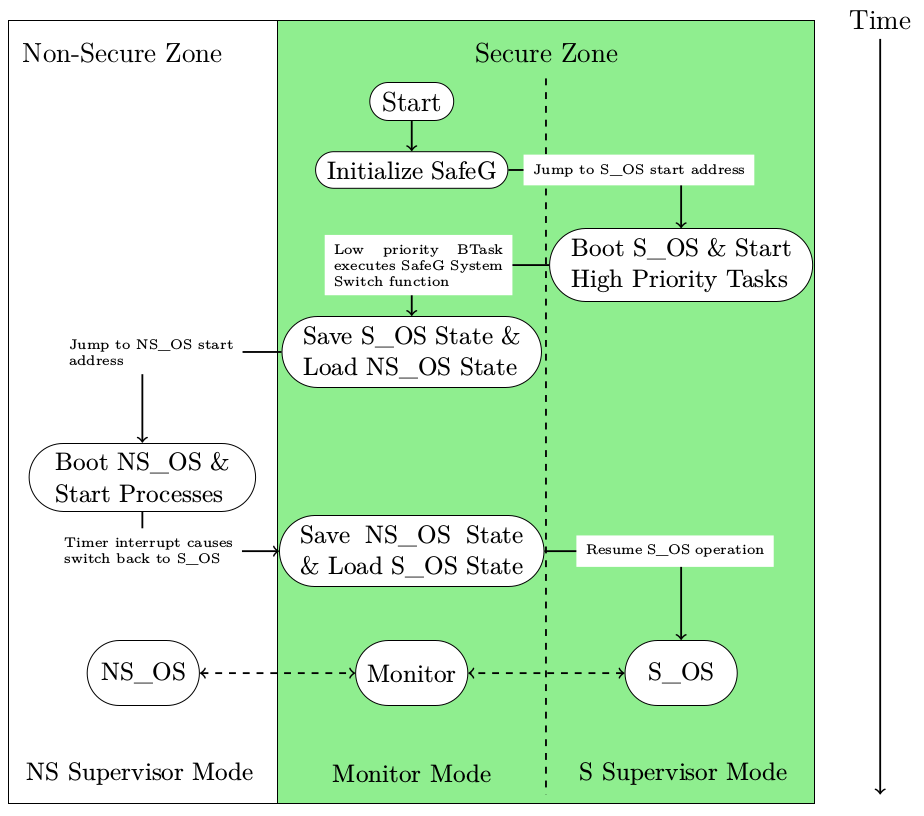
\includegraphics[width=\textwidth]{./img/literature_modeswitch.png}
%Flowchart of how the physical CPU switches between the virtual CPUs
\caption{Flowchart of the boot sequence of the CPU. \cite{zaki2016}}\label{fig:modeswitch}
\end{figure}

A Field Programmable Gate Array (FPGA) as interface between processor and board. Peripherals are separated as secure and non-secure using ARM TrustZone \cite{website:ARM}, see section~\ref{sec:trustzone}. \\ %TODO: Expand!

An overview of the system can be seen in Figure~\ref{fig:introduction_overview}.

\begin{figure}[H]
\centering
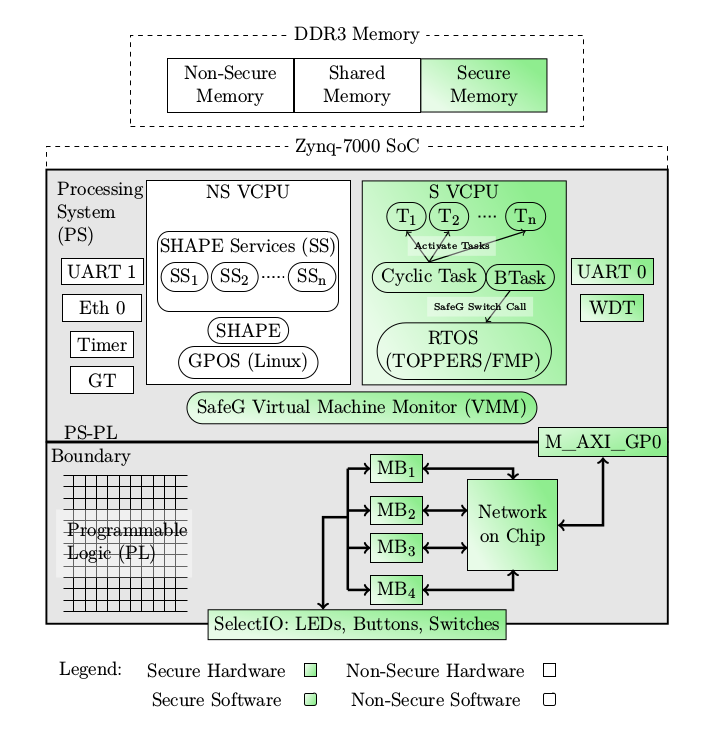
\includegraphics[width=\textwidth]{./img/introduction_overview.png}
\caption{System overview of the MCS in place.\cite{zaki2016}}\label{fig:introduction_overview}
\end{figure}

%Linux:
%Root File System
%Device Tree
%Kernel

%Boot SD:
%uboot

%FMP:
%compiled RTOS

\subsection{TrustZone}
\label{sec:trustzone}
"TrustZone is a security extension available in modern ARM processors that creates a security infrastructure designers can use to protect critical system assets. This infrastructure is achieved by enabling the partition of system components, both hardware and software, into either a Secure and a Normal world (or zone). Resources that are marked as normal are not permitted to access Secure zone components. This mechanism is enforced by the AMBA3 (Advanced Microcontroller Bus Architecture) AXI (Advanced eXtensible Interface) bus system. It contains an extra control signal for each of the read and write channels (Non-secure or NS bits) that dictate the access rights Non-secure bus masters to the Secure slaves. Each processor with an enabled TrustZone security extension can be partitioned into a Normal and a Secure virtual CPU. The virtual processors execute in a time-multiplexed fashion, and use the ”Monitor Mode” state to create an efficiently switching mechanism between Normal and Secure zones. The NS-bit, bit[0] of the Secure Configuration Register (SCR) in the System Control Coprocessor (CP15), controls the activation of secure state of the processor. Whenever the NS-bit set high, the processor state immediately switches to the Normal world. However, if the processor is in Monitor Mode, it remains in the Secure world regardless of the state of the SCR NS-bit. The processor state can nter monitor mode by either issuing a special instruction, SMC (Secure Monitor Call), in software or by hardware exception mechanisms such as IRQ, FIQ, external Data Abort, or external Prefetch Abort. In general, the software running in monitor mode serves the purpose of saving the state of the current world, and loading the state the other."~\cite{website:ARM} \\ %TODO: Wording

\section{Standards}
Safety practices are becoming more regulated as industries adopt a standardized set of practices for designing and testing products. %TODO: expand, wording

\subsection{IEC 61508}
IEC 61508~\cite{IEC61508} is intended to be a basic functional safety standard applicable to all kinds of industry. It defines four different safety integrity levels, SIL~1 being the least dependable up to SIL~4 which is the most dependable level.

\subsection{ISO 26262}
ISO 26262~\cite{ISO26262} addresses the needs for an automotive-specific international standard that focuses on safety critical components. ISO 26262 is a derivative of IEC 61508, the generic functional safety standard for electrical and electronic (E/E) systems.

\subsubsection{ASILs}
%ASIL QM (quality management) relates to the lowest (no) hazard, and ASIL
ISO 26262 describes five different levels relating to hazard and risk. Ranked from lowest (no) hazard to highest hazard: QM, A, B, C and D. A function is assigned an ASIL depending on the severity if the function fails, the probability that the function fails and the controllability of the function, see table~\ref{table:ASIL}.

\begin{table}[H]
\centering
\begin{tabular}{|c|c|c|c|c|}
\hline
\multirow{2}{*}{\textbf{Severity}} &\multirow{2}{*}{\textbf{Probability}} &\multicolumn{3}{|c|}{\textbf{Controllability}} \\ \cline{3-5}
 & &C1 &C2 &C3 \\ \hline
\multirow{4}{*}{S1} & E1 & QM & QM & QM \\ \cline{2-5}
 & E2 & QM & QM & QM \\ \cline{2-5}
 & E3 & QM & QM & A \\ \cline{2-5}
 & E4 & QM & A & B \\ \hline
\multirow{4}{*}{S2} & E1 & QM & QM & QM \\ \cline{2-5}
 & E2 & QM & QM & A \\ \cline{2-5}
 & E3 & QM & A & B \\ \cline{2-5}
 & E4 & A & B & C \\ \hline
\multirow{4}{*}{S3} & E1 & QM & QM & A \\ \cline{2-5}
 & E2 & QM & A & B \\ \cline{2-5}
 & E3 & A & B & C \\ \cline{2-5}
 & E4 & B & C & D \\ \hline
\end{tabular}
\caption{ASIL as a function of severity, probability and controllability.}
\label{table:ASIL}
\end{table}

The various integrity levels can be translated into integers (ASIL $QM = 0$; $A = 1$; $B = 2$; $C = 3$ and $D = 4$). If a hazard requires several components to fail, the added ASIL of these components is used to determine if there is an violation, assuming the components faults are statistically independent of each other. For example, a safety level ASIL B can be met by two independent components which each individually only meet ASIL A (and thus effectively $A + A = B$).~\cite{azevedo2014} \\ %TODO: semi Wording

The different ASILs relate to cost, see table~\ref{table:cost_heuritics}. % TODO: Expand, wording

\begin{table}[H]
\centering
\begin{tabular}{|c|c|c|c|c|c|}
\hline
\textbf{Cost Heuristic} & \textbf{QM} & \textbf{A} & \textbf{B} & \textbf{C} & \textbf{D} \\ \hline
Linear & 0 & 10 & 20 & 30 & 40 \\ \hline
Logarithmic & 0 & 10 & 100 & 1000 & 10000 \\ \hline
Experimental-I~\cite{azevedo2014} & 0 & 10 & 20 & 40 & 50 \\ \hline
Experimental-II~\cite{azevedo2014} & 0 & 20 & 30 & 45 & 55 \\ \hline
\end{tabular}
\caption{ASIL cost heuristics.}
\label{table:cost_heuritics}
\end{table}


\subsubsection{Freedom from interference}


\subsection{AUTOSAR}
"AUTOSAR (AUTomotive Open System ARchitecture) is a international development partnership of automotive interested parties founded in 2003. It pursues the objective of creating and establishing an open and standardized software architecture for automotive electronic control units (ECUs) excluding infotainment. Goals include the scalability to different vehicle and platform variants, transferability of software, the consideration of availability and safety requirements, a collaboration between various partners, sustainable utilization of natural resources, maintainability throughout the whole "Product Life Cycle"."~\cite{website:autosar}

The AUTOSAR Architecture distinguishes on the highest abstraction level between three software layers: Application, Runtime Environment (RTE) and Basic Software (BSW) which run on a Microcontroller.~\cite{website:autosar} See figure \ref{fig:autosar}.
\begin{itemize}
\item The application software layer is mostly hardware independent.
\item The RTE represents the full interface for applications.
\item The BSW is divided in three major layers and Complex Drivers: Services, ECU Abstraction and Microcontroller Abstraction. Services are divided furthermore into functional groups representing the infrastructure for System, Memory and Communication Services.
\end{itemize}

\begin{figure}[H]
\centering
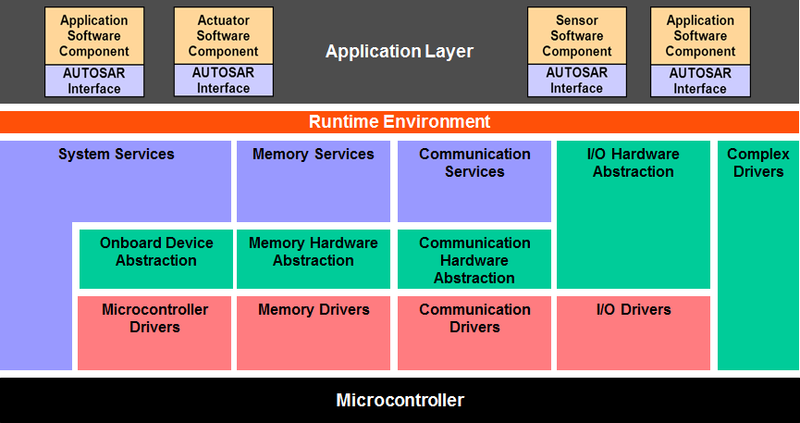
\includegraphics[width=\textwidth]{./img/literature_autosar.png}
\caption{AUTOSAR.~\cite{website:autosar}}\label{fig:autosar}
\end{figure}

